\documentclass[journal]{IEEEtran}

% *** GRAPHICS RELATED PACKAGES ***
%
\ifCLASSINFOpdf
   \usepackage[pdftex]{graphicx}
  % declare the path(s) where your graphic files are
  % \graphicspath{{../pdf/}{../jpeg/}}
  % and their extensions so you won't have to specify these with
  % every instance of \includegraphics
  % \DeclareGraphicsExtensions{.pdf,.jpeg,.png}
\else
  % or other class option (dvipsone, dvipdf, if not using dvips). graphicx
  % will default to the driver specified in the system graphics.cfg if no
  % driver is specified.
  % \usepackage[dvips]{graphicx}
  % declare the path(s) where your graphic files are
  % \graphicspath{{../eps/}}
  % and their extensions so you won't have to specify these with
  % every instance of \includegraphics
  % \DeclareGraphicsExtensions{.eps}
\fi

% correct bad hyphenation here
\hyphenation{op-tical net-works semi-conduc-tor}

\usepackage{threeparttable}
\usepackage{graphicx}
\usepackage{amsmath}
\usepackage{hyperref}
\renewcommand\figureautorefname{Fig.}
\hypersetup{
hidelinks,
% colorlinks=false,
% linkcolor=black
}
\usepackage{multirow}
\usepackage{booktabs}
\usepackage{marvosym}
\usepackage{subfigure}
% \usepackage{caption}
\usepackage{lipsum}
\usepackage{amsmath}
\begin{document}
%
% paper title
% Titles are generally capitalized except for words such as a, an, and, as,
% at, but, by, for, in, nor, of, on, or, the, to and up, which are usually
% not capitalized unless they are the first or last word of the title.
% Linebreaks \\ can be used within to get better formatting as desired.
% Do not put math or special symbols in the title.
\title{L-shape-based Block Partitioning and Iterative Prediction (L-BPIP) Algorithm for HEVC Intra-Frame Lossless Compression}
%
%
% author names and IEEE memberships
% note positions of commas and nonbreaking spaces ( ~ ) LaTeX will not break
% a structure at a ~ so this keeps an author's name from being broken across
% two lines.
% use \thanks{} to gain access to the first footnote area
% a separate \thanks must be used for each paragraph as LaTeX2e's \thanks
% was not built to handle multiple paragraphs
%

\author{
    Qinghao~Lin, Min~Lin\textsuperscript{\Letter}, Xiaoyu~Weng, Guojie~Chen
    %\IEEEmembership{Member,~IEEE,}
    %        John~Doe,~\IEEEmembership{Fellow,~OSA,}
    %        and~Jane~Doe,~\IEEEmembership{Life~Fellow,~IEEE}% <-this % stops a space

    \thanks{Q. Lin\IEEEauthorrefmark{1}, M. Lin\textsuperscript{\Letter} are with the Advanced SoC and IoT Technology Lab (ASITLAB), Key Laboratory of Specialty Fiber Optics and Optical Access Networks, Shanghai University, Shanghai 200444, China. (e-mail: shu\_rin@shu.edu.cn, mlin99@shu.edu.cn). (Corresponding author: Min Lin).}

    \thanks{This work was supported by Ministry of Science and Technology of China, through the National Key Research and Development Program of China, under Grant 2019YFB2204500.}
}


% note the % following the last \IEEEmembership and also \thanks - 
% these prevent an unwanted space from occurring between the last author name
% and the end of the author line. i.e., if you had this:
% 
% \author{....lastname \thanks{...} \thanks{...} }
%                     ^------------^------------^----Do not want these spaces!
%
% a space would be appended to the last name and could cause every name on that
% line to be shifted left slightly. This is one of those "LaTeX things". For
% instance, "\textbf{A} \textbf{B}" will typeset as "A B" not "AB". To get
% "AB" then you have to do: "\textbf{A}\textbf{B}"
% \thanks is no different in this regard, so shield the last } of each \thanks
% that ends a line with a % and do not let a space in before the next \thanks.
% Spaces after \IEEEmembership other than the last one are OK (and needed) as
% you are supposed to have spaces between the names. For what it is worth,
% this is a minor point as most people would not even notice if the said evil
% space somehow managed to creep in.


% The paper headers
%\markboth{IEEE TRANSACTIONS ON IMAGE PROCESSING,~VOL.~29, No.~8, August~2015}%
%{Shell \MakeLowercase{\textit{et al.}}: Bare Demo of IEEEtran.cls for IEEE Journals}
% The only time the second header will appear is for the odd numbered pages
% after the title page when using the twoside option.
% 
% *** Note that you probably will NOT want to include the author's ***
% *** name in the headers of peer review papers.                   ***
% You can use \ifCLASSOPTIONpeerreview for conditional compilation here if
% you desire.



% If you want to put a publisher's ID mark on the page you can do it like
% this:
%\IEEEpubid{0000--0000/00\$00.00~\copyright~2015 IEEE}
% Remember, if you use this you must call \IEEEpubidadjcol in the second
% column for its text to clear the IEEEpubid mark.


% use for special paper notices
%\IEEEspecialpapernotice{(Invited Paper)}



% make the title area
\maketitle
% As a general rule, do not put math, special symbols or citations
% in the abstract or keywords.
\begin{abstract}
    H.26x  family of video coding standards designed by ITU (International Telecom Union) is widely adopted in last decades, in which block-based prediction is employed in intra-frame coding. In this paper, we introduce an L-shape-based Block Partitioning and Iterative Prediction (L-BPIP) algorithm in which each block is divided into a series of close neighboring 1-D L-shapes and each L-shape prediction is performed by recursive method with previous neighboring L-shape as reference samples. When predicting each L-shape, similar to traditional block prediction, all the prediction modes are searched to find out the best one with minimum rate-distortion (RD) cost. Because of the L-shapes inherited close neighboring characteristics, L-shape-based iterative prediction can have much more accurate prediction results and much less residual bits which need to be coded and transmitted finally. In addition to smaller prediction residuals, ``Mode Residual'' is introduced so that most redundancy in increased number of mode information is eliminated due to iterative prediction method. To further maximize the efficiency of our prediction method, this paper also proposes an L-shape-based block partitioning method, which allows a block to be divided into a combination of an L-shaped block and a square block. Statistics shows this block partitioning method increases 15\% large blocks compared to traditional method, which can further reduce redundancy in mode information. Experimental results on HEVC reference software HM-16 shows that our proposed merge method is able to achieve an average of 8.87\% bit-rate saving, with the maximum of 14.14\% bit-rate saving on intra-frame lossless compression.
\end{abstract}

% Note that keywords are not normally used for peerreview papers.
\begin{IEEEkeywords}
    High efficiency video coding, intra-prediction, lossless coding, iterative prediction, mode residual, L-shape block partitioning, L-BPIP
\end{IEEEkeywords}




% For peer review papers, you can put extra information on the cover
% page as needed:
% \ifCLASSOPTIONpeerreview
% \begin{center} \bfseries EDICS Category: 3-BBND \end{center}
% \fi
%
% For peerreview papers, this IEEEtran command inserts a page break and
% creates the second title. It will be ignored for other modes.
\IEEEpeerreviewmaketitle


\section{Introduction}
% The very first letter is a 2 line initial drop letter followed
% by the rest of the first word in caps.
% 
% form to use if the first word consists of a single letter:
% \IEEEPARstart{A}{demo} file is ....
% 
% form to use if you need the single drop letter followed by
% normal text (unknown if ever used by the IEEE):
% \IEEEPARstart{A}{}demo file is ....
% 
% Some journals put the first two words in caps:
% \IEEEPARstart{T}{his demo} file is ....
% 
% Here we have the typical use of a "T" for an initial drop letter
% and "HIS" in caps to complete the first word.
\IEEEPARstart{H}{igh} Efficiency Video Coding (HEVC) standard is the most popular video coding standard of the Joint Collaborative Team on Video Coding (JCT-VC) \cite{01}. It can achieve about 50\% bit-rate saving in comparison with H.264/AVC \cite{02} for the same quality with a much higher coding complexity \cite{03}. It adopts various coding efficiency enhancement and parallel processing tools. The next generation Versatile Video Coding (VVC) \cite{a} standard developed by Joint Video Exploration Team (JVET) comes with a series of advanced coding tools in an effort to improve the coding efficiency \cite{b}, providing exceeding 30\% higher compression rate for the same video quality than HEVC. In several generations of the H.26x family of video coding standards designed by International Telecom Union (ITU) including H.265/HEVC and H.266/VVC, block-based prediction is performed in intra-prediction. This process performs angular and planar prediction to the current coding unit (CU) before which a frame is divided into CUs under a quadtree-based block partitioning structure.

In addition to the commonly used lossy video compression, lossless video compression is also very popular in many applications such as automotive vision, web collaboration, remote desktop sharing \cite{04}, content creation, post production, and professional applications such as medical imaging \cite{05}, and digital preservation in libraries and archives. Thus improving lossless intra-prediction coding efficiency is of great necessity.

To consider the lossless coding mode \cite{06}, we simply bypass transform, quantization, and in-loop filters (de-blocking filter, sample adaptive offset, and adaptive loop filter) \cite{07}.

In video codec standards, intra-prediction takes advantage of the correlation between adjacent pixels in the spatial domain to eliminate spatial redundancy in the image, and inter-prediction uses the correlation between adjacent frames in the temporal domain to eliminate temporal redundancy. Compared to inter-prediction, intra-prediction has great advantages of much simpler hardware structure and much lower power consumption, which is very suitable for the small and portable wearable devices such as light-weighted AR/VR devices. Intra-prediction is also used in the reference frame (I frame) of every Group Of Pictures (GOP) as an important part for inter-prediction. Further more, experimental results on the VVC platform VTM-12.0 shows that for intra-frame lossless compression, VVC provides only 10\% gain, with a price of much higher complexity which can be observed to have almost 25 times the encoding time compared to HEVC. That is a critical and detrimental flaw for low power and real-time performance required by wearable AR/VR devices, increasing the significance of improving HEVC intra-frame lossless compression. 

For intra-prediction, HEVC block-based prediction can provide accurate prediction because of its flexible block partitioning method, but in the case of predicting large blocks, pixels close to the edge of the block which are far away from the reference samples will inevitably produce larger prediction residuals, resulting in the reduce of the coding efficiency. Secondly, although the traditional block partitioning method can provide an appropriate partitioning result, some of the sub blocks under the same parent block cannot be jointly predicted and coded when there appears some kind of texture mutation in the parent block, even if they choose the same prediction mode and share a common texture. This can cause the problem of increasing redundancy of mode and partitioning information.

Due to these imperfections of traditional algorithm, we design an L-shape-based Block Partitioning and Iterative Prediction (L-BPIP) algorithm in this paper to improve intra-frame lossless compression in HEVC. The main contributions of this work are as follows:

\begin{itemize}
    \item [1)]
          Propose a new iterative prediction method.
    \item [2)]
          A new L-shape-based block partitioning method is introduced.
    \item [3)]
          Based on the two points above, we propose an L-shape-based Block Partitioning and Iterative Prediction (L-BPIP) algorithm.
\end{itemize}

\begin{figure*}[tp]
    \centering
    \includegraphics[width=14cm]{pictures/HEVCprediction.pdf}
    \caption{Traditional angular prediction in HEVC}
    \label{fig:HEVCprediction}
\end{figure*}

The iterative prediction method can decrease the minimum distance between the reference samples and the predicted samples, thereby reducing prediction residuals. And by introducing L-shape blocks, we can merge regions with similar textures so that the region containing rich textures can still maintain blocks as large as possible locally, only using small blocks for coding in the highly detailed texture regions. Simultaneously, the form of the L-shape block can better fit the iterative prediction we proposed and further reduce the redundancy in mode information. Through the combination of the two methods, the so-called L-shape-based Block Partitioning and Iterative Prediction (L-BPIP) algorithm is presented for better performance in the intra-frame lossless compression.

The rest of this paper is organized as follows. Section II provides a review of traditional intra-prediction and block partitioning method in HEVC. Section III introduced the proposed L-shape-based Iterative Prediction (L-IP) and L-shape-based Block Partitioning (L-BP) method in detail, as well as the overall framework process of their combined implementation. Section IV introduces the optimization of the scheme and analyzes its effect. Section V provides the experimental results with analysis and discussion. Finally, Section VI concludes this paper.

\begin{figure}[tp]
    \centering
    \includegraphics[width=8.8cm]{pictures/residual}
    \caption{Average prediction distortions of all 35 intra modes in 16 × 16 PUs}

    \label{fig:residual}
\end{figure}
\section{ANALYSIS OF INTRA PREDICTION AND BLOCK PARTITIONING IN HEVC AND RELATED WORK}

\subsection{INTRA PREDICTION IN HEVC}
Intra-prediction is one of the core parts of video coding. This process uses prediction residuals to replace the pixel data which need to be coded and transmitted so as to perform data compression.

\autoref{fig:HEVCprediction} shows an example of traditional angular prediction in HEVC. For each certain angular direction, the decoded and reconstructed samples of the nearest neighboring blocks are used as reference samples. Pixels are projected along the angular direction associated with the intra mode to the reference line to get its predicted value. If it doesn't fall on integer grid, the linear interpolations of neighboring reference samples of the intersection are used to generate the predicted value in 1/32 pixel precision:
\begin{equation}
    P_{(x,y)} =((32-w)\cdot R_{(0,i)} +w\cdot R_{(0,i+1)} +16)>>5
\end{equation}
where we denote reference sample by $R_{(x,y)}$, and predicted sample by $P_{(x,y)}$. The subscript, $(x,y)$, represents the coordinates of the pixel, which defines the top-left pixel as $(0,0)$. If some reference samples, like $R_{(N+1,0)}$~$R_{(2N,0)}$ are missing due to prediction order or location of the current CU (such as the picture/slice boundaries), they need to be padded with the nearest available reference sample before the predicting process. $w$ in the function denotes the weight of the reference samples depends on the position of the projection point.

Although in this process, the nearest reference lines along the current block are used, it is the block-based feature that makes the pixels near the edge of the block farther from the reference line which results in the inaccurate predicted value in this area and thus leads to larger prediction residuals. \autoref{fig:residual} displays the average prediction distortions of all 35 intra modes in 16 × 16 luma prediction units (PUs) \cite{08}. These statistical results are generated by encoding 1st frames of four sequences (Traffic, Kimono, BasketballDrill, and FourPeople) using HM-16.12. Dark area means a small distortion, and bright area represents a high distortion level. It can be clearly observed from the experimental results shown in \autoref{fig:residual} that, when the distance becomes longer between the pixel and the reference line, the residuals goes up simultaneously. Smaller prediction residuals are located in the region close to the reference line, while the intra prediction is inferior in the farther regions, which is caused by the attenuation of spatial correlation as the prediction distance ascends.

For this flaw of intra-prediction, \cite{d} presented a intra coding method based on sample-by-sample differential pulse code modulation (DPCM), which applies DPCM on residuals after intra prediction and it is used for only lossless coding in H.264/AVC Fidelity Range Extensions (FRExt). And HEVC had modification compared to H.264/AVC FRExt, supporting horizontal and vertical DPCM coding modes for residual signals (with either intra-prediction or inter-prediction) in HEVC Range Extension (RExt) \cite{e, h}. This kind of pixel-by-pixel DPCM is also named as residual DPCM (RDPCM) since DPCM is applied to the residuals \cite{i}.
 \cite{09} introduced a sample-based angular intra prediction (SAP) method, which employed the same prediction mode signalling method and the sample interpolation method as the HEVC block-based angular prediction, but uses adjacent neighbors for better intra prediction accuracy and performs prediction sample by sample. Subsequent DPCM-based proposals are SAP-HV \cite{10}, SAP1 \cite{11}, and SAP-E \cite{12}. SAP-HV applies DPCM exclusively in the pure horizontal and vertical directions. SAP1 is similar to SAP but employs a more uniform density of prediction modes in the vertical and horizontal directions. SAP-E has been shown to provide further bit-rate reductions over SAP, SAP-HV and SAP1, as tested on large color biomedical images \cite{12}. \cite{13} analyzed the range of values in residual blocks and apply accordingly a pwm function to map specific residual values to unique lower values and encode appropriate parameters associated with the pwm functions at the encoder, so that the corresponding inverse pwm functions at the decoder can map values back to the same residual values. \cite{14} exploited inter-channel correlation using reconstructed luma to predict chroma linearly with parameters derived from neighboring reconstructed luma and chroma pixels at both encoder and decoder to avoid overhead signalling. Cross-Component Linear Model (CCLM) for chroma intra-prediction is a promising coding tool in Joint Exploration Model (JEM) developed by the Joint Video Exploration Team (JVET). \cite{15} introduced an approach which can classify neighboring luma and chroma samples of the current block into several groups, and derive a particular set of linear model parameters for each group, and a new prediction method synthesizing the angular intra-prediction and the MM-CCLM intra-prediction into a new chroma intra coding mode. \cite{16} made full use of reconstructed pixels to predict later ones in bidirectional or multi-directional manner by coding pixels alternately with interleave prediction. In \cite{17}, to reduce residual energy, half pixels are coded via a novel padding technique together with a constrained quantization algorithm, whereas the other half are reconstructed by linear interpolations along a prediction direction by utilizing the neighboring reference pixels and the first half coded pixels. To alleviate the encoder computational load, \cite{18} proposed an adaptive mode decision algorithm based on texture complexity and direction for HEVC intra prediction to filter out unnecessary coding block. The original redundant mode candidates for each PU are reduced according to its texture direction. In \cite{19}, to solve the two issues: the incoherence caused by the signal noise or the texture of other objects, and that the nearest reference line usually has worse reconstruction quality in block-based video coding, it proposed an multiple-line-based intra-prediction scheme to improve coding efficiency. Besides the nearest reference line, further reference lines are also utilized. The further reference lines with a relatively higher quality can provide potentially better prediction. At the same time, the residue compensation is introduced to calibrate the prediction of boundary regions in a block when we utilize further reference lines.

In these works, though SAP \cite{09}-\cite{12} can solve the problem of the long distance between reference samples and predicted samples, the RD cost is calculated based on the whole block because only one prediction mode is allowed in one block, which still hindering the block partitioning process from generating the most appropriate result for rich texture area. What's more, the SAP series of algorithms cannot be used in the lossy compression because the sample by sample method results in the diability in reconstruction, which is of great importance in lossy mode in HEVC.

\begin{figure}[tp]
    \centering
    \subfigure[]{
    \includegraphics[width=3cm]{pictures/l-shaped block illustration a.pdf}
    }
    \subfigure[]{
    \includegraphics[width=3cm]{pictures/l-shaped block illustration b.pdf}
    }
    \caption{Example of quadtree-based block partitioning with high textured content in a relatively flat block overall of RaceHorses (a) expected partitioning result in HEVC (b) expected partitioning result in proposed L-shaped block partitioning method}
    \label{fig:l-shaped block}
\end{figure}

\subsection{QUADTREE-BASED BLOCK PARTITIONING IN HEVC}
HEVC expands the 16 × 16 macroblock size used by the H.264/AVC standard to 64 × 64, which enables regions with simple textures or relatively static regions to be predicted and encoded in larger blocks, saving partitioning information and mode information overhead, so as to improve the coding efficiency . HEVC proposes the concepts of Coding Tree Unit (CTU) and CU to replace macroblocks, and adopts the quadtree-based block partitioning method to perform more accurate block partitioning result matching on different texture details. For area with rich textures, using smaller blocks for prediction can get smaller prediction residuals, but will result in more partitioning and mode information; regions with simple textures use larger blocks for prediction, which can save a certain amount of additional information, but at the same time the prediction distortion rises. This problem becomes more serious in regions farther away from the reference samples, like the block boundary. Therefore, we need to find a balance between more additional information and better prediction accuracy. The criterion used in HEVC is the rate- distortion optimization (RDO) between the prediction accuracy and the bit cost. The RD cost function (Jmode) used in HM is evaluated as follows \cite{17}
\begin{equation}
    J_{mode}=B_{mode}+\lambda_{mode}\cdot SSE
\end{equation}
Where B$_{mode}$ specifies bit cost to be considered for mode decision, which depends on each decision case. Sum of Squared Error (SSE) is the average difference between reconstructed CU and the matching blocks, $\lambda_{mode}$ is the Lagrange multiplier. In lossless case, the function will be
\begin{equation}
    J_{mode}=B_{mode}
    \label{RDo}
\end{equation}
because no more distortion is produced when bypassing transform, quantization, and in-loop filters. In a block, RDO process is used to search for the best prediction mode (with the minimum RD cost) and the best block partitioning result.

In the process, a frame is first divided into several CTUs of the same size. Each CTU is the largest coding unit where RDO process is performed from the bottom to the top to determine the final block partitioning result. \autoref{fig:l-shaped block}(a) shows an example of a CTU after block partitioning process. Each square represents an independent CU/PU (the two concept of CU and PU in this paper will not cause any obstacles to understanding, they all refer to a block to be predicted, coded and transmitted). HEVC uses a split flag to indicate whether a block is split to the next depth. After the block partitioning process, each CU performs prediction independently within itself.

It can be observed that under the quadtree-based block partitioning structure, since each block performs prediction independently, joint prediction is not allowed in the sub blocks under the same parent block even if they uses the same prediction mode. This causes unnecessary mode information. As shown in \autoref{fig:l-shaped block}, due to the high textured content in a very small area in the lower right corner of the current block, the entire CTU is divided into 16 blocks The number may be, 12 or even smaller if we can merge these sub blocks together. This situation directly leads to a decline in compression performance.

\begin{figure*}[htpb]
    \centering
    \includegraphics[width=14cm]{pictures/Lprediction.pdf}
    \caption{(a) Proposed L-shape-based iterative prediction process stopping at the last L-shape (b) Schematic diagram of different projection offset of neighboring prediction mode}
    \label{fig:comparison}
\end{figure*}

Because of the high computational complexity in the implementation of quadtree-based block partitioning in HEVC, some works so far have tried to simplify the partitioning procedure. Cao et al. \cite{20} proposed a short distance intra prediction (SDIP) based on the quadtree block partitioning structure, improving the intra prediction accuracy by splitting a coding unit into nonsquare units for coding and reconstruction. To decrease the coding complexity, memory access, and power consumption, which go against its widely applications, especially for ultra-high definition and/or mobile video applications, \cite{21} proposed approaches consisting two stages of support vector machine-based fast INTRA CU size decision schemes at four CU decision layers to early terminate CU splitting or early skip checking the current CU depth. \cite{22} allowed for significant reduction in computational complexity with small degradations in RD performance containing two complementary steps: 1) early CU split decision and 2) early CU pruning decision. The early CU splitting and pruning tests are performed at each depth level to avoid unnecessary calculation of RD cost. Choi et al. \cite{23} proposed a new bottom-up-based block partitioning method called split-and-merge. This method splits an image into multiple square blocks and merges them into nonsquare blocks to exploit the dependence between split blocks. Moreover, a modification of the conventional intra prediction and transform is employed for nonsquare blocks. \cite{24} proposed a coding framework supporting hierarchical splitting with binary and ternary trees and flexible coding order representations. The proposed compression scheme provides significantly higher compression capability than the state-of-the-art HEVC/H.265 standard for Standard Dynamic Range (SDR) category while maintaining complexity acceptable for emerging applications.

In other respects, \cite{25} analyzed the problem with the current lossless coding scheme and propose a mode-dependent template (MD-template) based method for intra lossless coding.In order to achieve higher transform coding gains with relatively low-complexity implementations, \cite{26} propose a joint separable and non-separable transform, which is named Enhanced Multiple Transform (EMT), applying multiple transform cores from a pre-defined subset of sinusoidal transforms, and the transform selection is signalled in a joint block level manner. \cite{27} focused on CNN technology joining with image restoration to facilitate video
coding performance, and propose the content-aware CNN based in-loop filtering for HEVC. \cite{28} redesigned the intra mode coding method based on both short and long range correlations, as the existing approaches based on local content correlations cannot always effectively capture the most probable mode. And it achieved unified content adaptive coding and is applicable across different video content.

However, most works above are performed under the premise of the structure of binary, ternary or quad trees, and do not really solve the above problem described in Part B.


\section{PROPOSED LOSSLESS INTRA-PREDICTION}
As analyzed in Section II, two reasons motivate us to conduct this study: 1) The block-based prediction in HEVC results in inaccuracy of the prediction on the edge far away from the reference line of the block thus cannot accurately match the rich texture and 2) the generation of mode information redundancy because sub blocks under the same parent block cannot be predicted jointly.

In this section, we first introduce two proposed methods in details and then we present a merge method to maximize their gain.

% Please add the following required packages to your document preamble:
% \usepackage{multirow}
\begin{table*}[]
    \centering
    \caption{residual reduction of L-IP}
    \label{table: residual reduction}
    \begin{tabular}{c|c|c|c|c|c|c|c}
        \toprule
        \multirow{2}{*}{Class}                          & \multirow{2}{*}{Sequence}    & \multicolumn{2}{c|}{4 × 4}   & \multicolumn{2}{c|}{8 × 8}  & \multicolumn{2}{c}{16 × 16}                             \\ \cline{3-8}
                                                        &                              & HEVC                         & L-IP                         & HEVC                        & L-IP    & HEVC    & L-IP    \\ \hline
        \multirow{2}{*}{Class B}                        & BasketballDrive              & 30.01                        & 26.54                       & 130.94                      & 116.08 & 536.56  & 401.07 \\ \cline{2-8}
                                                        & Kimono                       & 27.39                        & 20.58                       & 100.63                      & 86.52  & 371.53  & 291.05 \\ \hline
        Class C                                         & PartyScene                   & 109.97                       & 98.62                       & 463.98                      & 316.04 & 1067.07 & 860.59 \\  \hline
        Class E                                         & Johnny                       & 27.85                        & 17.23                       & 82.54                       & 60.19  & 230.74  & 164.25 \\ \hline
        Class F                                         & SlideEditing                 & 163.6                        & 135.32                      & 337.67                      & 248.71 & 1464.68 & 560.35 \\ \hline
        \multicolumn{2}{c|}{AVG reduction   percentage} & \multicolumn{2}{c|}{20.43\%} & \multicolumn{2}{c|}{22.14\%} & \multicolumn{2}{c}{31.36\%}                                                           \\ \bottomrule
    \end{tabular}
    % \begin{tablenotes}
    %     \footnotesize
    %     \item[1]The number of blocks of size 32 × 32 is very small thus is not statistically significant.
    % \end{tablenotes}
\end{table*}

\subsection{L-SHAPE-BASED ITERATIVE PREDICTION (L-IP)}
To overcome the first issue mentioned above, an L-shape-based Iterative Prediction (L-IP) method for HEVC lossless intra-prediction is provided. The core idea is to split a block into a series of close neighboring 1-D L-shapes and each L-shape prediction is performed by recursive method with previous neighboring L-shape as reference samples from top left to bottom right.

% Please add the following required packages to your document preamble:
% \usepackage{multirow}
\begin{table*}[]
    \centering
    \caption{partitioning result comparison of L-shape-based iterative prediction (L-IP) and block-based prediction (BP)}
    \label{table: partitioning result}
    \begin{tabular}{c|c|cc|cc|cc|cc}
        \toprule
        \multirow{2}{*}{Class}                                  & \multirow{2}{*}{Sequence}     & \multicolumn{2}{c|}{4 × 4}   & \multicolumn{2}{c|}{8 × 8}   & \multicolumn{2}{c|}{16 × 16} & \multicolumn{2}{c}{32 × 32}                                       \\
                                                                &                               & L-IP                         & BP                           & L-IP                         & BP                          & L-IP    & BP     & L-IP    & BP     \\ \hline
        \multirow{2}{*}{Class A}                                & PeopleOnStreet                & 19.27\%                      & 90.24\%                      & 5.58\%                       & 8.24\%                      & 28.21\% & 1.45\% & 46.94\% & 0.07\% \\
                                                                & Traffic                       & 14.93\%                      & 87.80\%                      & 4.22\%                       & 11.46\%                     & 29.50\% & 0.70\% & 51.35\% & 0.05\% \\ \hline
        \multirow{2}{*}{Class B}                                & BasketballDrive               & 48.44\%                      & 63.73\%                      & 22.78\%                      & 26.49\%                     & 16.30\% & 9.36\% & 12.48\% & 0.43\% \\
                                                                & BQTerrace                     & 42.09\%                      & 72.62\%                      & 11.98\%                      & 15.54\%                     & 19.79\% & 7.61\% & 26.14\% & 4.22\% \\ \hline
        \multicolumn{2}{c|}{AVG reduction/increment percentage} & \multicolumn{2}{c|}{-47.42\%} & \multicolumn{2}{c|}{-4.29\%} & \multicolumn{2}{c|}{18.67\%} & \multicolumn{2}{c}{33.04\%}                                                                      \\ \bottomrule
    \end{tabular}
    % \begin{tablenotes}
    %     \footnotesize
    %     \item[1]The partitioning results in row 3-6 denote the percantage of the pixel numbers of all the N × N blocks in pixel numbers of the whole frame.
    % \end{tablenotes}
\end{table*}

For a block of size N × N, we split it into N-1 L-shapes and one pixel (at the bottom right corner). As is shown in \autoref{fig:comparison}(a), the first L-shape, L1, is predicted in the same way as HEVC, using the decoded and reconstructed samples of the nearest neighboring blocks (L0) as reference samples. Other L-shapes with m pixels use the decoded and reconstructed pixels of the closest neighboring L-shape which has m+2 pixels as reference line. Except for the reference samples, the generation of the predicted value is almost the same as in HEVC which calculates the linear interpolations of two reference samples neighbor to the intersection of the projection line and the reference line:
\begin{equation}
    P_{(x,y)}^{Lj} =((32-w)\cdot R_{(0,i)}^{Lj-1} +w\cdot R_{(0,i+1)}^{Lj-1} +16)>>5
\end{equation}
where the subscript, $(x,y)$, represents the coordinates of the pixel in the current L-shape, which defines the top-left pixel as $(0,0)$, and the superscript, $Li$, represents the number of the L-shape.
Unlike in HEVC, we just need to pad (copy) one pixel at the two ends of each reference line like $R_{(0,N)}^{L1},R_{(0,N-1)}^{L2}$ because as shown in \autoref{fig:comparison}(a). The maximum distance between the projection position and the edge of the reference line will be less than one pixel wide.

We can also see clearly from \autoref{fig:HEVCprediction} and \autoref{fig:comparison} that the distance between current position (yellow dots) and the reference sample (gray dots) in block-based prediction in HEVC is becoming longer while the position is closer to the right and the lower boundary. But in the proposed L-IP, the distance won't change with the position under a apecific prediction angle.

To demonstrate that the L-IP can reduce the residual energy, we provide some statistics of the average residual obtained by the two prediction methods in the case of the same block size. We study the $1^{st}$ frame of of Class B sequences (BasketballDrive and Kimono), Class C sequence (PartyScene), Class E sequence (Johnny) and Class F sequences. \autoref{table: residual reduction} shows that the average prediction residual is reduced by 20.43\% in blocks of size 4 × 4, 22.14\% in blocks of size 8 × 8 and 31.36\% in blocks of size 16 × 16 (The number of blocks of size 32 × 32 is very small thus is not statistically significant).

\begin{figure*}[tp]
    \centering
    \includegraphics[width=14cm]{pictures/partitioning process.pdf}
    \caption{Block Partitioning result (a) Quadtree-based in traditional HEVC (b) Proposed l-shaped (c) Overall process of block partitioning from the block of size 8 × 8 to 32 ×32}
    \label{fig:partitioning}
\end{figure*}
After the process of L-IP, The pixels on the same L-shape will share the same prediction mode, so there are N prediction modes for a block of size N × N. Obviously, to encode and transmit these data directly will be an extra cost. Based on the strong correlation between adjacent pixels and blocks in the image picture, we can reasonably assume that in most cases, the prediction modes of adjacent L-shapes should be the same or only varies in a quite small range. ``Mode Residual'' is thus introduced to eliminate most redundancy in increased number of mode information due to iterative prediction method. It refers to encoding and transmitting only the variation of these N modes. In addition, it is easy to find that in HEVC, when the size of the block is small enough (for example, 4 × 4), the block-based prediction is accurate enough. If we still perform L-IP until the last L-shape, even if we can provide much more accurate prediction, the gain of that may be offset by the redundancy due to extra mode information, and it may even leads to worse overall performance. After statistical experiments on the HEVC test sequence, we found that keeping a base block in L-IP as 4 × 4 can save unnecessary expenses and provide the best performance. In the base block we still adopt L-IP except that there is only one prediction mode in the base block. In other words, every L-shape use the same prediction mode to generate the predicted value and the RDO process is also block-based. In this way, we can inhibit the generation of mode residuals as far as possible while ensuring the prediction accuracy.

Another improvement aim at L-IP is the number reduction of the prediction modes which is reduced from 35 modes to 8 modes. As is shown in \autoref{fig:comparison}(b), we can see that the offset of the projection between the neighboring angle mode is becoming smaller while the distance between the reference sample and the predicted sample. So using such high-density distributed angle modes is unnecessary for L-IP and will cause extra mode information. And the experimental data shows that the number reduction enabled in L-IP can even bring over 1\% bit-rate saving.

Furthermore, in addition to the increase in prediction accuracy due to the shorter distance to the reference sample, there is another benefit that can be expected. For block-based prediction, a block can only have one certain prediction mode, this will results in an increase in the proportion of small blocks in the result of the block partitioning result for regions with rich textures. In L-IP, every L-shape can have its own separate prediction mode so that it can get more accurate prediction for rich textures within a larger block more accurately. This characteristic should be manifested as a large increase in the number of large blocks in the block partitioning result. It has also been verified in experiments shown in \autoref{table: partitioning result} (The partitioning results in row 3-6 denote the percantage of the pixel numbers of all the N × N blocks in pixel numbers of the whole frame). The proportion of blocks of size 16 × 16 and 32 × 32 is increased by 18.67\% and 33.04\% while that of size 4 × 4 and 8 × 8 is decreased by 47.42\% and 4.29\% respectively. Intuitively, with more larger blocks, more partitioning and mode information redundancy is eliminated, which can further help improve the performance of L-IP.


\begin{figure*}[tp]
    \centering
    \includegraphics[width=18cm]{pictures/flowchart.pdf}
    \caption{Flowchart of the proposed L-BPIP in HEVC lossless intra-prediction}
    \label{fig:flowchart}
\end{figure*}
\subsection{L-SHAPE-BASED BLOCK PARTITIONING (L-BP)}
As mentioned in the previous section, sub blocks under the same parent block can't be predicted jointly in traditional HEVC algorithm. Once there is high textured content in the current block, there is a high probability that it will be split into 4 sub blocks. Extra mode information will be generated in those sub blocks that don't contain rich textures. \autoref{fig:l-shaped block} shows this situation. Because some high textured contents exist at the lower-right corner, the whole block of size 64 × 64 is split into 16 blocks. This can be worse especially when using L-IP method because one more block of size N × N means N-2 more mode residuals. Considering this situation and the shape characteristics of L-IP, we propose an L-shape-based Block Partitioning (L-BP) method. In this way, we can ensure the retention of the larger blocks while there has a high textured content, so as to fully remove the redundancy of the mode information and further maximize the gain of L-IP. The so-called L-shaped block partitioning is to treat a block as two parts: the L-shaped part and the reserved block part. This process is equivalent to merge the three of the sub blocks together as the L-shaped block for joint prediction after the block partitioning process using traditional HEVC method. Since the high textured content mentioned earlier may occur anywhere in the current block, the reserved block is allowed to be located on 4 corners in this algorithm, namely upper left, upper right, lower left, and lower right.

For the reserved block, we expect to retain the block partitioning results of previous depth level, otherwise repartitioning will cause huge amount of unnecessary overhead. A contradiction occurs here that during the basis for judging whether a block should be split in HEVC: RDO process. $B_{mode}$ in \eqref{RDo} contains the bit cost of the mode information, the partitioning information and the bit cost of transmitting the encoded residual data, so the mode and partitioning information generated during block partitioning will affect the bit cost after encoding, thereby changing the final RD cost. Once the RD cost changed, the final partitioning result will also change.

In HEVC, mode information will not be transmitted directly. For pictures and videos, the high correlation between neighboring blocks results in a high probability that the intra prediction modes of adjacent blocks will be the same or similar. Therefore, the HEVC standard construct a modes list including two most probable modes (MPMs) and additional probable intra modes when intra mode coding \cite{18}. There are 3 candidate modes which are used to store the prediction modes of spatially nearby blocks (the above block and the left block).

Based on the analysis above, if we want to retain the results of the previous depth level, once the prediction modes of the blocks nearby changes, the MPM will also change, resulting in the different value of the RD cost and finally leads to different partitioning results of the reserved block. This may even lead to wrong mode information decoded by the decoder and cause serious distortion. This is equivalent to overturning the original partitioning result which we want to retain.

For these reasons, we are to ignore the inaccuracy in RD cost, re-construct MPMs and recode the mode information after the block partitioning result is completely determined. Because the main factor that determines the result of the block partitioning is the texture characteristics of the image in the current block, it is reasonable to speculate that the impact to the block partitioning result of directly ignoring the inaccurate RD cost caused by the mode information can be ignored.

In order to verify the feasibility of this method, we compare the RD cost of the blocks of size 4 × 4 and 8 × 8 with the recalculated RD cost after the reserving process is completed. Experimental result shows that for the reserved blocks, the difference between the two RD cost is $\pm$0.27\% for 4 × 4 blocks and $\pm $0.29\% for 8 × 8 blocks in average, which can almost be ignored.

The overall process of block partitioning uses the same bottom-up approach as in HEVC. The method we proposed is equivalent to adding a splicing step on the basis of the traditional block partitioning result. \autoref{fig:partitioning} shows the splicing process. \autoref{fig:partitioning}(a) shows the partitioning result in traditional HEVC; \autoref{fig:partitioning}(b) shows the L-shaped block partitioning result after the splicing process; \autoref{fig:partitioning}(c) shows the bottom-up comparison process. Starting from the smallest block of size 4 × 4 (case 4 × 4 is omitted in the figure owing to space constraints), the comparing process is performed in each level of depth, and finally determine the block partitioning result of the entire CTU.

\subsection{L-SHAPE-BASED BLOCK PARTITIONING AND ITERATIVE PREDICTION (L-BPIP)}
According to the aforementioned analysis, combining the two methods together can maximize their advantages. There- fore, we propose a merge method that combines L-BP and L-IP called L-shape-based Block Partitioning and Iterative Prediction (L-BPIP) algorithm to replace the one in traditional HEVC intra-frame lossless compression. We use the same criterion of block partitioning: RDO process. For any input CU, the RDO process will be performed under 11 cases (shown in \autoref{fig:eleven}) and the best case (with minimum RD cost) is chosen to construct the final partitioning result.

\begin{figure}[tp]
    \centering
    \includegraphics[width=8.8cm]{pictures/eleven cases.pdf}
    \caption{Cases of a block to be compared in the RDO process}
    \label{fig:eleven}
\end{figure}

Since there are 11 situations to be compared, directly transmitting will require 4bit-wide data. We have found that in these cases, three account for most of the proportions (``split to next depth'' accounts for 61\%, ``lower-right reserved BP'' accounts for 9\% and ``lower-right reserved L-IP'' accounts for 9\%). So we decide to use variable length coding (VLC) to save the redundancy in partitioning information. \autoref{fig:flowchart} shows a flowchart of the proposed overall algorithm, where Rd\_* means different RD cost to be compared during the whole process, Rd\_nons means the RD cost of non-split blocks, Rd\_split means the one of four sub blocks under the current block. Rd\_res means the RD cost of blocks have reserved blocks in it, Rd\_blk means the RD cost of blocks using block-based prediction while Rd\_L\_sum means the sum of the RD cost of L-shapes and base blocks using L-IP, Rd\_res\_i means the RD cost of four cases of reserving-based intra prediction.

\begin{figure}[tp]
    \centering
    \includegraphics[width=8.8cm]{pictures/special.pdf}
    \caption{Two special cases of L-IP in L-BPIP}
    \label{fig:special}
\end{figure}

During the L-IP performed to the L-shaped block in this merge method, in order to uniform the overall process, we adopt the same prediction order from the upper-left L-shape to the lower-right L-shape for all four reserved cases. Except that the case in the upper-left reserved which predict the reserved block first and the L-shapes later, and the case in the lower-right reserved which predict the L-shapes first and the reserved block later, other three cases may have special prediction order in L-IP to solve the problem of missing reconstructed reference samples, which are discussed here:

\begin{itemize}
    \item [1)]
          Upper-left reserved: first predict and reconstruct the re- served block, and then perform L-shape-based iterative prediction to the remaining pixels.
    \item [2)]
          Upper-right or lower-left reserved: the prediction order is L1 → L2 → L3 → L4 → B1 → B2.
    \item [3)]
          Lower-right reserved: the prediction order is L1 → L2 → L3 → L4 → reserved block.
\end{itemize}
The schematic diagram of the prediction process is shown in \autoref{fig:special}.

At the decoding side, we have the same order as the encoding side, we use the decoded and reconstructed result of it as reference samples and do iterative prediction to the next neighboring L-shape. For the special cases above, the algorithm iterates in the order: L1 → L2 → L3 → L4 → B1 → B2.

In this prediction and decoding order, we can make sure that before every block or L-shape is predicted, the reference samples it needs are already reconstructed.

\begin{figure*}[tp]
    \begin{equation}
        P_{(x,y)}=\left\{
        \begin{aligned}
            min(R_{(x,y-1)},R_{(x-1,y)})          &  & if R_{(x-1,y-1)} \geq max(R_{(x,y-1)},R_{(x-1,y)}) \\
            max(R_{(x,y-1)},R_{(x-1,y)})          &  & if R_{(x-1,y-1)} \leq min(R_{(x,y-1)},R_{(x-1,y)}) \\
            R_{(x,y-1)}+R_{(x-1,y)}-R_{(x-1,y-1)} &  & otherwise
        \end{aligned}
        \right.
        \label{planar}
    \end{equation}
\end{figure*}

\begin{figure}[tp]
    \centering
    \includegraphics[width=4 cm]{pictures/optimization.pdf}
    \caption{The RD cost calculation order in the case of upper-right reserved-BP}
    \label{fig:optimization}
\end{figure}


% Please add the following required packages to your document preamble:
% \usepackage{multirow}
\begin{table*}[tp]
    \centering
    \caption{LOSSLESS CODING PERFORMANCE COMPARISON OF THE PROPOSED METHODS IN TERMS OF BIT-RATE DIFFERENCES WITH RESPECT TO HEVC ALL-INTRA UNDER LOSSLESS CONFIGURATION}
    \label{table:final}
    \begin{tabular}{c|c|c|c|cccc}
        \toprule
        \multirow{2}{*}{Class}                            & \multirow{2}{*}{Sequence} & L-IP     & L-BP                       & \multicolumn{4}{c}{L-BPIP}                                                        \\
                                                          &                           & All      & All                       & Y                          & Cb       & Cr                  & All                 \\ \midrule[1pt]
        \multirow{2}{*}{\begin{tabular}[c]{@{}c@{}}Class A\\ (2560 × 1600)\end{tabular}}       & PeopleOnStreet            & -11.29\% & -1.78\%                   & -14.03\%                   & -13.86\% & -11.43\%            & -13.42\%            \\
                                                          & Traffic                   & -11.46\% & -1.89\%                   & -14.30\%                   & -9.60\%  & -13.98\%            & -13.26\%            \\ \hline
        \multirow{5}{*}{\begin{tabular}[c]{@{}c@{}}Class B\\ (1080p)\end{tabular}}       & BasketballDrive           & -4.20\%  & -2.28\%                   & -2.74\%                    & -3.72\%  & -9.90\%             & -4.30\%             \\
                                                          & BQTerrace                 & -8.57\%  & -1.80\%                   & -9.32\%                    & -7.40\%  & -7.84\%             & -9.12\%             \\
                                                          & Cactus                    & -3.74\%  & -1.15\%                   & -3.76\%                    & -2.84\%  & -5.34\%             & -3.92\%             \\
                                                          & Kimono                    & -7.71\%  & -1.57\%                   & -6.74\%                    & -13.72\% & -21.14\%            & -9.07\% (-7.57\%)   \\
                                                          & ParkScene                 & -6.58\%  & -1.48\%                   & -7.50\%                    & -9.36\%  & -10.43\%            & -7.95\% (-8.27\%)   \\ \hline
        \multirow{4}{*}{\begin{tabular}[c]{@{}c@{}}Class C\\ (WVGA)\end{tabular}}       & BasketballDrive           & -5.51\%  & -1.96\%                   & -2.81\%                    & -2.06\%  & -4.63\%             & -3.76\%             \\
                                                          & BQMall                    & -6.17\%  & -1.46\%                   & -5.80\%                    & -7.06\%  & -10.91\%            & -6.55\%             \\
                                                          & PartyScene                & -5.58\%  & -1.42\%                   & -5.27\%                    & -6.74\%  & -8.30\%             & -5.71\%             \\
                                                          & RaceHorses                & -8.10\%  & -1.46\%                   & -8.14\%                    & -14.89\% & -15.70\%            & -9.21\%             \\ \hline
        \multirow{4}{*}{\begin{tabular}[c]{@{}c@{}}Class D\\ (WQVGA)\end{tabular}}       & BasketballPass            & -12.36\% & -2.62\%                   & -13.02\%                   & -16.15\% & -17.76\%            & -13.79\%            \\
                                                          & BlowingBubbles            & -5.47\%  & -1.05\%                   & -4.89\%                    & -8.35\%  & -11.11\%            & -5.42\%             \\
                                                          & BQSquare                  & -5.27\%  & -1.54\%                   & -4.37\%                    & -6.20\%  & -8.33\%             & -5.05\%             \\
                                                          & RaceHorses                & -8.51\%  & -1.17\%                   & -8.58\%                    & -13.80\% & -14.54\%            & -9.38\%             \\ \hline
        \multirow{3}{*}{\begin{tabular}[c]{@{}c@{}}Class E\\ (720p)\end{tabular}}       & FourPeople                & -12.51\% & -3.52\%                   & -11.43\%                   & -23.62\% & -22.93\%            & -14.14\%            \\
                                                          & Johnny                    & -10.97\% & -4.11\%                   & -9.15\%                    & -20.92\% & -20.63\%            & -12.29\%            \\
                                                          & KristenAndSara            & -11.86\% & -4.40\%                   & -10.44\%                   & -21.16\% & -20.91\%            & -13.24\%            \\ \midrule[1pt]
        \multicolumn{2}{c|}{Average of Class A - Class E} & -8.10\%                   & -2.04\%  & -7.90\%                   & -11.19\%                   & -13.10\% & -8.87\%                                   \\ \midrule[1pt]
        \multirow{4}{*}{\begin{tabular}[c]{@{}c@{}}Class F\\ (screen content)\end{tabular}}       & BasketballDrillText       & -6.07\%  & -1.96\%                   & -3.39\%                    & -3.30\%  & -5.83\%             & -4.50\% (-6.38\%)   \\
                                                          & ChinaSpeed                & -17.15\% & -4.75\%                   & -19.37\%                   & -15.40\% & -16.22\%            & -18.56\% (-14.42\%) \\
                                                          & SlideEditing              & -13.57\% & -2.64\%                   & -16.86\%                   & -8.24\%  & -9.54\%             & -15.49\% (-11.80\%) \\
                                                          & SlideShow                 & -22.26\% & -5.43\%                   & -25.25\%                   & -26.96\% & -26.22\%            & -26.42\% (-18.92\%) \\ \midrule[1pt]
        \multicolumn{2}{c|}{Average of Class F}           & -14.76\%                  & -3.70\%  & -16.22\%                  & -13.48\%                   & -14.45\% & -16.24\% (-12.88\%)                       \\ \midrule[1pt]
        \multicolumn{2}{c|}{Average of All}               & -9.31\%                   & -2.34\%  & -9.42\%                   & -11.61\%                   & -13.35\% & -10.21\%                                  \\ \midrule[1pt]
        \multicolumn{2}{c|}{Encoding time}                & 125\%                     & 101\%    & \multicolumn{4}{c}{129\%}                                                                                     \\ \midrule[1pt]
        \multicolumn{2}{c|}{Decoding time}                & 103\%                     & 100\%    & \multicolumn{4}{c}{103\%}                                                                                     \\ \bottomrule
    \end{tabular}
    \begin{tablenotes}
        \footnotesize
        \item[1]Results in parenthesis \cite{13} indicate the benefits of SAP-E \cite{12}       with respect to HEVC all-intra under lossless configuration.
    \end{tablenotes}

\end{table*}



\begin{figure*}[tp]
    \centering
    \subfigure[block partitioning results in HEVC using traditional prediction and partitioning method]{
            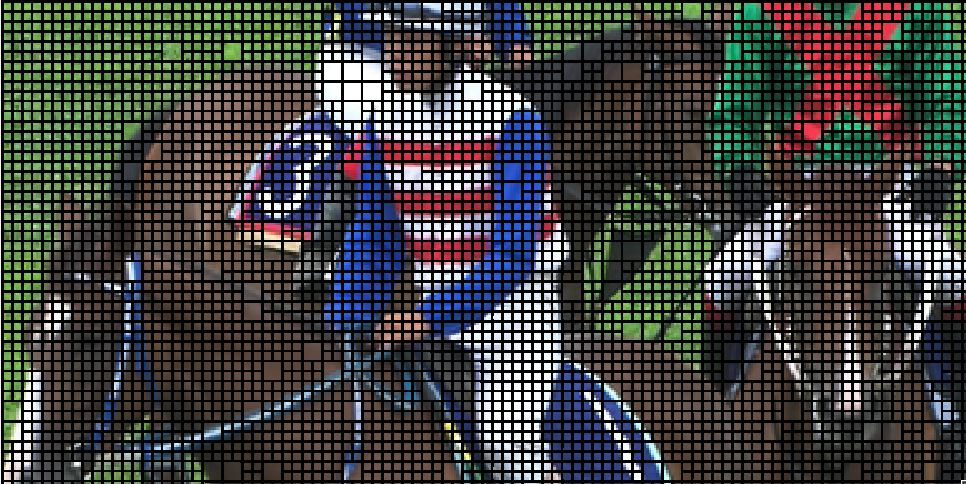
\includegraphics[width=11cm]{pictures/RaceHorseshevc}
    }
    \subfigure[block partitioning results using proposed L-BPIP]{
            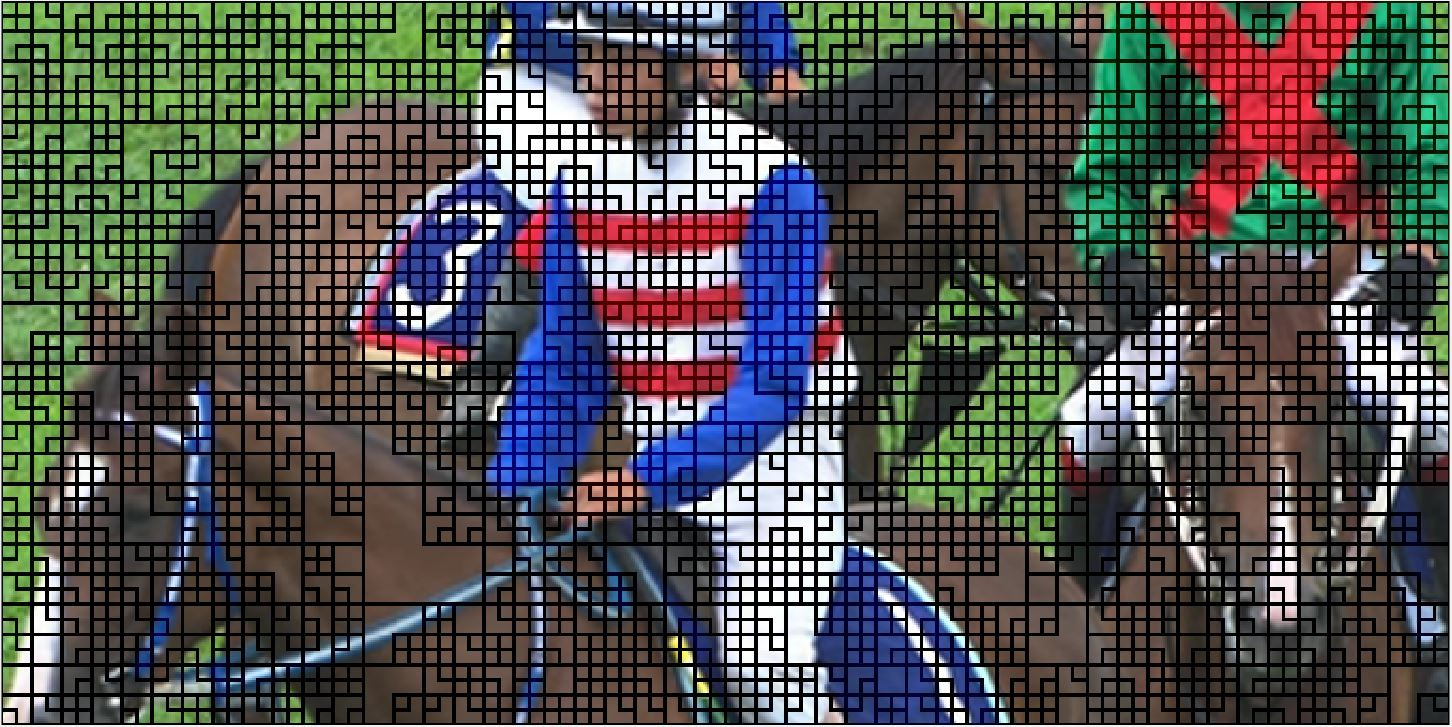
\includegraphics[width=11cm]{pictures/RaceHorsesnew}
    }
    \caption{Block partitioning result comparison of the proposed L-BPIP with respect to HEVC all-intra under lossless configuration}
    \label{fig:HEVC block}
\end{figure*}

\section{IMPLEMENTATION AND OPTIMIZATION}

In the implementation of RDO, HEVC always encodes the residual coefficient in the size of 4 × 4 for all block size when transmitting, so the RD cost can be considered as the sum of RD costs of 4 × 4 units. For example, the RD cost of the 8 × 8 block is the sum of B1, B2, B3 and B4 though predicted in a whole block in \autoref{fig:optimization}. For HEVC uses context-based adaptive binary arithmetic coding (CABAC) to encode the data need to be transmitted, the context-based characteristic of it leads to different results of RD cost if the coding order is changed.

As \autoref{fig:optimization} shows, in the case of upper-right reserved-BP, the coding order for the L-shape block is B1 → B3 → B4. B2 is missing because the reserved block needs to be processed separately. This results in the changing context of B3, and different encoding result and RD cost at the meantime. So in former L-BPIP, the L-shape block of four reserved cases need to be recoded to ensure the correct RD cost. This process is actually ineffective and it increases the encoding time. The reason is that the L-shape block and the square block use the same reference sample during block-based prediction, which leads to the same predicted value for the pixels in the same position and it can be reasonably assumed that the difference of the RD cost due to the changing context can be ignored.

So we proposed the scheme to reduce the encoding time. During the RDO process of the case that having L-shape blocks and choose block-based prediction, we directly use the four RD costs generated in the block-based predicted CU where the L-shape block is located and calculate the sum of three of them (in \autoref{fig:optimization}, the three is the RD cost of B1, B3 and B4, they are generated during the 8 × 8 block is predicted as a whole using block-based prediction) according to which position the reserved block is as the RD cost of the L-shape block. This optimization can save the block-based prediction and encoding process for L-shape blocks.

Furthermore, to maximize the benefits of reducing the distance between the reference samples and predicted sample, we apply SAP-E \cite{12} in planar prediction mode, in which the predicted value is calculated as \eqref{planar} \cite{29}.

%where b denotes $R_{(x,y-1)}$, c denotes $R_{(x-1,y-1)}$ and d denotes $R_{(x-1,y)}$. 
And sample by sample method is performed to horizon (mode 10) and vertical (mode 26) prediction mode.

\section{EXPERIMENTAL RESULTS}
To verify the effectiveness of the proposed method, we perform the experiment in the HEVC reference software HM-16. We take the whole range of HEVC test sequences as our test sequence. There are six classes containing five natural video classes and one screen content class: Class A (2560 × 1600); Class B (1080p); Class C (WVGA); Class D (WQVGA); Class E (720p); Class F (screen content). The experiment strictly follows the HEVC common test condition (CTC) \cite{31}. The bit-rate gain is used to assess the coding performance of the proposed methods, where a negative number indicates bit-rate saving. Since our methods are designed for lossless intra-coding, we only test the lossless All Intra (AI) configuration in HM. \autoref{table:final} shows the coding performance of the proposed three intra-frame lossless compression for the three luma and chroma components and the whole gain compared with the original coding method in HEVC for each sequence under lossless AI. The encoding and decoding time are tabulated in the last two lines. We use the following $\Delta T$ to calculate the encoding or decoding time difference,
\begin{equation}
    \Delta T=\frac{T_{proposed}}{T_{anchor}} \times 100\%
\end{equation}
where $T_{proposed}$ means the encoding time or decoding time of the proposed method, $T_{anchor}$ means the encoding or decoding time of the original HEVC method in HM-16.
\subsection{L-shape-based Iterative Prediction (L-IP)}
The experiment result for L-IP is shown in the third column of \autoref{table:final}. For L-IP, the maximum bit-rate saving is 12.51\% for FourPeople in Class A - Class E, and 22.26\% for SlideShow in Class F, with an average of 8.10\% for Class A - Class E and 14.76\% for Class F. For computational complexity, L-IP is observed to increase the encoding time by 25\%, with almost the same decoding time.
 
\subsection{L-shape-based Block Partitioning (L-BP)}
As shown in the fourth column of \autoref{table:final}, the maximum bit-rate saving of L-BP is 4.40\% for KristenAndSara in Class A - Class E, and 5.43\% for SlideShow in Class F, with an average of 2.04\% for Class A - Class E and 3.70\% for Class F. For this method, both the encoding and decoding time have barely changed.
\subsection{L-shape-based Block Partitioning and Iterative Prediction (L-BPIP)}
Column 5-8 of \autoref{table:final} shows the gain of L-BPIP which has the best performance of the three proposed methods. The maximum bit-rate saving is 14.14\% for FourPeople in Class A - Class E, and 26.42\% for SlideShow in Class F, with an average of 8.87\% for Class A - Class E and 16.24\% for Class F. L-BPIP is observed to increase the encoding time by 29\%, with almost the same decoding time. This level of increase in encoding time is objectively acceptable for this degree of computational complexity.

\subsection{Comparison to SAP-E}
In HEVC intra-frame lossless compression, The SAP series of algorithms have the highest benefits in the published literature in our knowledge. Among them, SAP-E \cite{12} perform the best efficiency. Let us recall that though SAP series of algorithms use sample by sample method in prediction, in RDO process, they still take blocks as units, which affect the accuracy of the block partitioning. L-BPIP use several L-shape and allow them to have different prediction mode to avoid the problem. In \cite{12}, it test only part of HEVC test sequences: Class B-ParkScene,Class B-Kimono, and Class F. It can be seen in \autoref{table:final} that the bit-rate saving of L-BPIP is increased by 0.59\% and 3.36\% with comparison to SAP-E in the average benefit of Class A - Class E and Class F.
\subsection{Further analysis}
From the statistics above, we can observe that compared with L-IP and L-BP, the bit-rate saving of L-BPIP is increase by 0.89\% and 7.87\%, which proves the significance and necessity of combining L-IP and L-BP. In the meantime, compared with the block partitioning result in traditional HEVC method, the proportion of 16 × 16 and 32 × 32 blocks of L-BPIP is increased by 25.82\% (shown in \autoref{fig:HEVC block}), which confirms our conjecture that the intra-frame lossless compression coding using the combination of L-IP and L-BP can increase the number of larger blocks, which provides L-IP with favourable conditions. It is easy to imagine that the larger the current block is, the greater the gain brought by the use of L-IP will be, because it can save a considerable part of mode information generated in the traditional method, while ensuring the same or even better accuracy of the prediction.

Further more, it is worth noting that, although L-BPIP needs to compare 11 cases during RDO process, the encoding time only increases by less than 1 time. As is analyzed in section III, part B, the RD cost of 5 cases concluding Block-based prediction (BP) among all the 11 cases can be directly obtained from the result of the previous depth level because we retain the partitioning results instead of repartitioning. That's the main reason of the reducing encoding time. Another reason is that in RDO process,we use the bit cost of the original prediction residual instead of the one of the encoded prediction residual.
\section{conclusion}
In this paper, we proposed a new prediction method and a new block partitioning method to increase the coding efficiency for HEVC intra-frame lossless compression. First, we design an L-shape-based iterative prediction to decrease residual instead of traditional block-based prediction. Secondly, an L-shape-based block partitioning method is presented to take full advantage of the new prediction method and reduce mode information redundancy. The experiment results show that the proposed new methods can provide up to 14.14\% bit rate reduction with an average of 8.87\% and we adopt some implementation optimization to speed up the whole prediction and RDO process,increasing the encoding time by only 29\% when it is enabled, which is acceptable for process of this complexity.

\ifCLASSOPTIONcaptionsoff
    \newpage
\fi

% references section

% can use a bibliography generated by BibTeX as a .bbl file
% BibTeX documentation can be easily obtained at:
% http://mirror.ctan.org/biblio/bibtex/contrib/doc/
% The IEEEtran BibTeX style support page is at:
% http://www.michaelshell.org/tex/ieeetran/bibtex/
%\bibliographystyle{IEEEtran}
% argument is your BibTeX string definitions and bibliography database(s)
%\bibliography{IEEEabrv,../bib/paper}
%
% <OR> manually copy in the resultant .bbl file
% set second argument of \begin to the number of references
% (used to reserve space for the reference number labels box)
\bibliographystyle{IEEEtran}
\bibliography{ref}

% \begin{thebibliography}{11}
%     \bibitem{01}G. J. Sullivan, J. Ohm, W. Han and T. Wiegand, ``Overview of the High Efficiency Video Coding (HEVC) Standard,'' in IEEE Transactions on Circuits and Systems for Video Technology, vol. 22, no. 12, pp. 1649-1668, Dec. 2012.
%     \bibitem{02}Advanced Video Coding, ISO/IEC Standard 14496-10:2009, Mar. 2010.
%     \bibitem{03}J. Ohm, G. J. Sullivan, H. Schwarz, T. K. Tan and T. Wiegand, ``Comparison of the Coding Efficiency of Video Coding Standards—Including High Efficiency Video Coding (HEVC),'' in IEEE Transactions on Circuits and Systems for Video Technology, vol. 22, no. 12, pp. 1669-1684, Dec. 2012.
%     \bibitem{04}Z. Pan, H. Shen, Y. Lu, S. Li and N. Yu, ``A Low-Complexity Screen Compression Scheme for Interactive Screen Sharing,'' in IEEE Transactions on Circuits and Systems for Video Technology, vol. 23, no. 6, pp. 949-960, June 2013
%     \bibitem{05}V. Sanchez and J. Bartrina-Rapesta, ``Lossless compression of medical images based on HEVC intra coding,'' 2014 IEEE International Conference on Acoustics, Speech and Signal Processing (ICASSP), Florence, 2014.
%     \bibitem{06}X. Jizheng, R. Joshi, and R.A. Cohen, ``Overview of the Emerging HEVC Screen Content Coding Extension,'' IEEE Transactions on Circuits and Systems for Video Technology, vol. 26, no. 1, pp. 50-62, Jan. 2016.
%     \bibitem{07}M. Mrak and J. Xu, ``Improving screen content coding in HEVC by transform skipping,'' in Proc. of the 20th European Signal Processing Conference (EUSIPCO), 2012, pp. 1209-1213.
%     \bibitem{08}K. Fan, R. Wang, G. Li and W. Gao, ``Efficient Prediction Methods With Enhanced Spatial-Temporal Correlation for HEVC,'' in IEEE Transactions on Circuits and Systems for Video Technology, vol. 29, no. 12, pp. 3716-3728, Dec. 2019.
%     \bibitem{09}M. Zhou, W. Gao, M. Jiang, and H. Yu, ``HEVC lossless coding and improvements,'' IEEE Trans. Circuits and Systems for Video Tech., vol. 22, no. 12, pp. 1839-1843, Dec. 2012.
%     \bibitem{10}M. Zhou and M. Budagavi, ``RCE2: Experimental results on Test 3 and Test 4,'' Joint Collaborative Team on Video Coding (JCT-VC), Doc. JCTVC-M0056, Incheon, Korea, Nov. 2013.
%     \bibitem{11}V. Sanchez, J. Bartrina-Rapesta, F. Aulí-Llinàs, and J. Serra-Sagristà, ``Improvements to HEVC Intra Coding for Lossless Medical Image Compression,'' in Proc. 2014 Data Compression Conference (DCC), March 2014, pp. 423.
%     \bibitem{12}V. Sanchez, F. Aulí-Llinàs, J. Bartrina-Rapesta and J. Serra-Sagristà, ``HEVC-based Lossless Compression of Whole Slide Pathology Images,'' in Proc. 2014 IEEE Global Conference on Signal and Information Processing (GlobalSIP), pp. 452-456, Dec. 2014.
%     \bibitem{13}V. Sanchez, F. Aulí-Llinàs and J. Serra-Sagristà, ``Piecewise Mapping in HEVC Lossless Intra-Prediction Coding,'' in IEEE Transactions on Image Processing, vol. 25, no. 9, pp. 4004-4017, Sept. 2016.
%     \bibitem{14}X. Zhang, C. Gisquet, E. François, F. Zou and O. C. Au, ``Chroma Intra Prediction Based on Inter-Channel Correlation for HEVC,'' in IEEE Transactions on Image Processing, vol. 23, no. 1, pp. 274-286, Jan. 2014.
%     \bibitem{15}K. Zhang, J. Chen, L. Zhang, X. Li and M. Karczewicz, ``Enhanced Cross-Component Linear Model for Chroma Intra-Prediction in Video Coding,'' in IEEE Transactions on Image Processing, vol. 27, no. 8, pp. 3983-3997, Aug. 2018.
%     \bibitem{16}V. Sanchez, ``Lossless screen content coding in HEVC based on sample-wise median and edge prediction,'' 2015 IEEE International Conference on Image Processing (ICIP), Quebec City, QC, 2015.
%     \bibitem{17}C. Chen, S. Zhu, B. Zeng and M. Gabbouj, ``A New Block-Based Method for HEVC Intra Coding,'' in IEEE Transactions on Circuits and Systems for Video Technology, vol. 27, no. 8, pp. 1727-1736, Aug. 2017.
%     \bibitem{18}X. Liu, Y. Liu, P. Wang, C. Lai and H. Chao, ``An Adaptive Mode Decision Algorithm Based on Video Texture Characteristics for HEVC Intra Prediction,'' in IEEE Transactions on Circuits and Systems for Video Technology, vol. 27, no. 8, pp. 1737-1748, Aug. 2017.
%     \bibitem{19}J. Li, B. Li, J. Xu and R. Xiong, ``Efficient Multiple-Line-Based Intra Prediction for HEVC,'' in IEEE Transactions on Circuits and Systems for Video Technology, vol. 28, no. 4, pp. 947-957, April 2018.
%     \bibitem{20}X. Cao, C. Lai, Y. Wang, L. Liu, J. Zheng and Y. He, ``Short Distance Intra Coding Scheme for High Efficiency Video Coding,'' in IEEE Transactions on Image Processing, vol. 22, no. 2, pp. 790-801, Feb. 2013.
%     \bibitem{21}Y. Zhang, Z. Pan, N. Li, X. Wang, G. Jiang and S. Kwong, ``Effective Data Driven Coding Unit Size Decision Approaches for HEVC INTRA Coding,'' in IEEE Transactions on Circuits and Systems for Video Technology, vol. 28, no. 11, pp. 3208-3222, Nov. 2018.
%     \bibitem{22}S. Cho and M. Kim, ``Fast CU Splitting and Pruning for Suboptimal CU Partitioning in HEVC Intra Coding,'' in IEEE Transactions on Circuits and Systems for Video Technology, vol. 23, no. 9, pp. 1555-1564, Sept. 2013.
%     \bibitem{23}B. Choi and S. Ko, ``Split-and-Merge-Based Block Partitioning for High Efficiency Image Coding,'' in IEEE Transactions on Circuits and Systems for Video Technology, vol. 28, no. 2, pp. 540-549, Feb. 2018.
%     \bibitem{24}K. Choi et al., ``Video Codec Using Flexible Block Partitioning and Advanced Prediction, Transform and Loop Filtering Technologies,'' in IEEE Transactions on Circuits and Systems for Video Technology, vol. 30, no. 5, pp. 1326-1345, May 2020.
%     \bibitem{25}Z. Gu, W. Lin, B. Lee, C. T. Lau and M. Sun, ``Mode-Dependent Templates and Scan Order for H.264/AVC-Based Intra Lossless Coding,'' in IEEE Transactions on Image Processing, vol. 21, no. 9, pp. 4106-4116, Sept. 2012.
%     \bibitem{26}X. Zhao, J. Chen, M. Karczewicz, A. Said and V. Seregin, ``Joint Separable and Non-Separable Transforms for Next-Generation Video Coding,'' in IEEE Transactions on Image Processing, vol. 27, no. 5, pp. 2514-2525, May 2018.
%     \bibitem{27}C. Jia et al., ``Content-Aware Convolutional Neural Network for In-Loop Filtering in High Efficiency Video Coding,'' in IEEE Transactions on Image Processing, vol. 28, no. 7, pp. 3343-3356, July 2019.
%     \bibitem{28}J. Li et al., ``Unified Intra Mode Coding Based on Short and Long Range Correlations,'' in IEEE Transactions on Image Processing, vol. 29, pp. 7245-7260, 2020.
%     \bibitem{29}M. Weinberger, G. Seroussi and G. Sapiro, ``The LOCO-I lossless image compression algorithm: Principles and standardization into JPEG-LS'', IEEE Trans. Image Process, pp. 1309-1324, Aug. 2000.
%     \bibitem{30}HM15.0 software. [Online]. Available: https://vcgit.hhi.fraunhofer.de/jct-vc/HM
%     \bibitem{31}F. Bossen, Common HM Test Conditions and Software Reference Configurations, ITU-T/ISO/IEC Joint Collaborative Team on Video Coding (JCT-VC), document Rec. JCTVC-L1100, 2013.
% \end{thebibliography}

\end{document}

